\label{sec:seismic}

%\tcb{first draft C Mow-Lowry/G Losurdo Nov 2019}

{\bf Overview of seismic isolation}

The seismic isolation system fulfills three main functions:
\begin{itemize}
    \item to suppress the seismic noise below the sensitivity requirements in the detection frequency range (for ET at frequencies larger than 1-2 Hz);
    \item to reduce the RMS input motion to the suspension systems, particularly at the suspension resonances and the micro-seismic peak(s);
    \item to provide large-scale and slow position control of the test-masses.
\end{itemize}

Two main concepts have been implemented so far in GW ground-based detectors:
\begin{itemize}
    \item The Virgo Superattenuator \cite{};
    \item The Advanced LIGO HEPI/ISI \cite{}.
\end{itemize}

Both of them rely on a combination of passive and active isolation, but the approach is substantially different. The Superattenuator is mostly based on a passive approach to seismic noise suppression, thanks to a design characterized by very low normal mode frequencies, whereas it needs active control for RMS reduction. On the contrary, the Advanced LIGO system makes use of an aggressive control strategy to "dig" actively into the seismic noise.


{\bf ET baseline}

The baseline for ET, defined in the 2011 CDR and detailed there, consists in using a longer Virgo-style Superattenuator. The increased length (17 m) allows to reduce the normal mode frequencies and push the seismic wall down to $\sim$2 Hz. 

The main advantage for such a choice is that it provides a design thoroughly tested during many years of operation in Virgo and which requires only minor R\&D to be adapted to ET: it therefore represents a safe pathway towards a 3G configuration. 

\paragraph{SA modifications for Low Frequency ET}

In order to extend the detection bandwidth of the Einstein Telescope in the low-frequency region starting from a couple of Hz, a better seismic attenuation in the ultra-low frequency range is needed. To this purpose a detailed simulation devoted to this design study was performed for the 2011 ET Conceptual Design. The SA dynamics in the low frequency range, where the inner normal modes of the mechanical filter chain are confined, was simulated by using the electro-magnetic equivalent circuit (a series of oscillators). 
A maximization algorithm, called \emph{Simplex}~\cite{Different2008_SecondEdition}, based on the possibility to change the masses and the mechanical filter chain lengths, was developed. It searches for a maximum attenuation performance at a fixed frequency that, in our case, was 2\,Hz.  Since the transfer function has a smooth shape, it turns out that to get a higher attenuation at 2\,Hz, we should have a lower  "cross-over frequency" with the requirements curves (see Fig.~\ref{Par4Fig1}). As showed in the direct measurement performed with the Virgo interferometer (see section 4.1.1.c), the cross-over between seismic noise at the mirror level and the requirements is dominated by the residual horizontal seismic vibrations. For this reason to move the cross-over at lower frequency, we need to improve  the attenuation performance of the horizontal seismic vibration in the low frequency range.
%
\begin{figure}[t]
	\begin{center}
		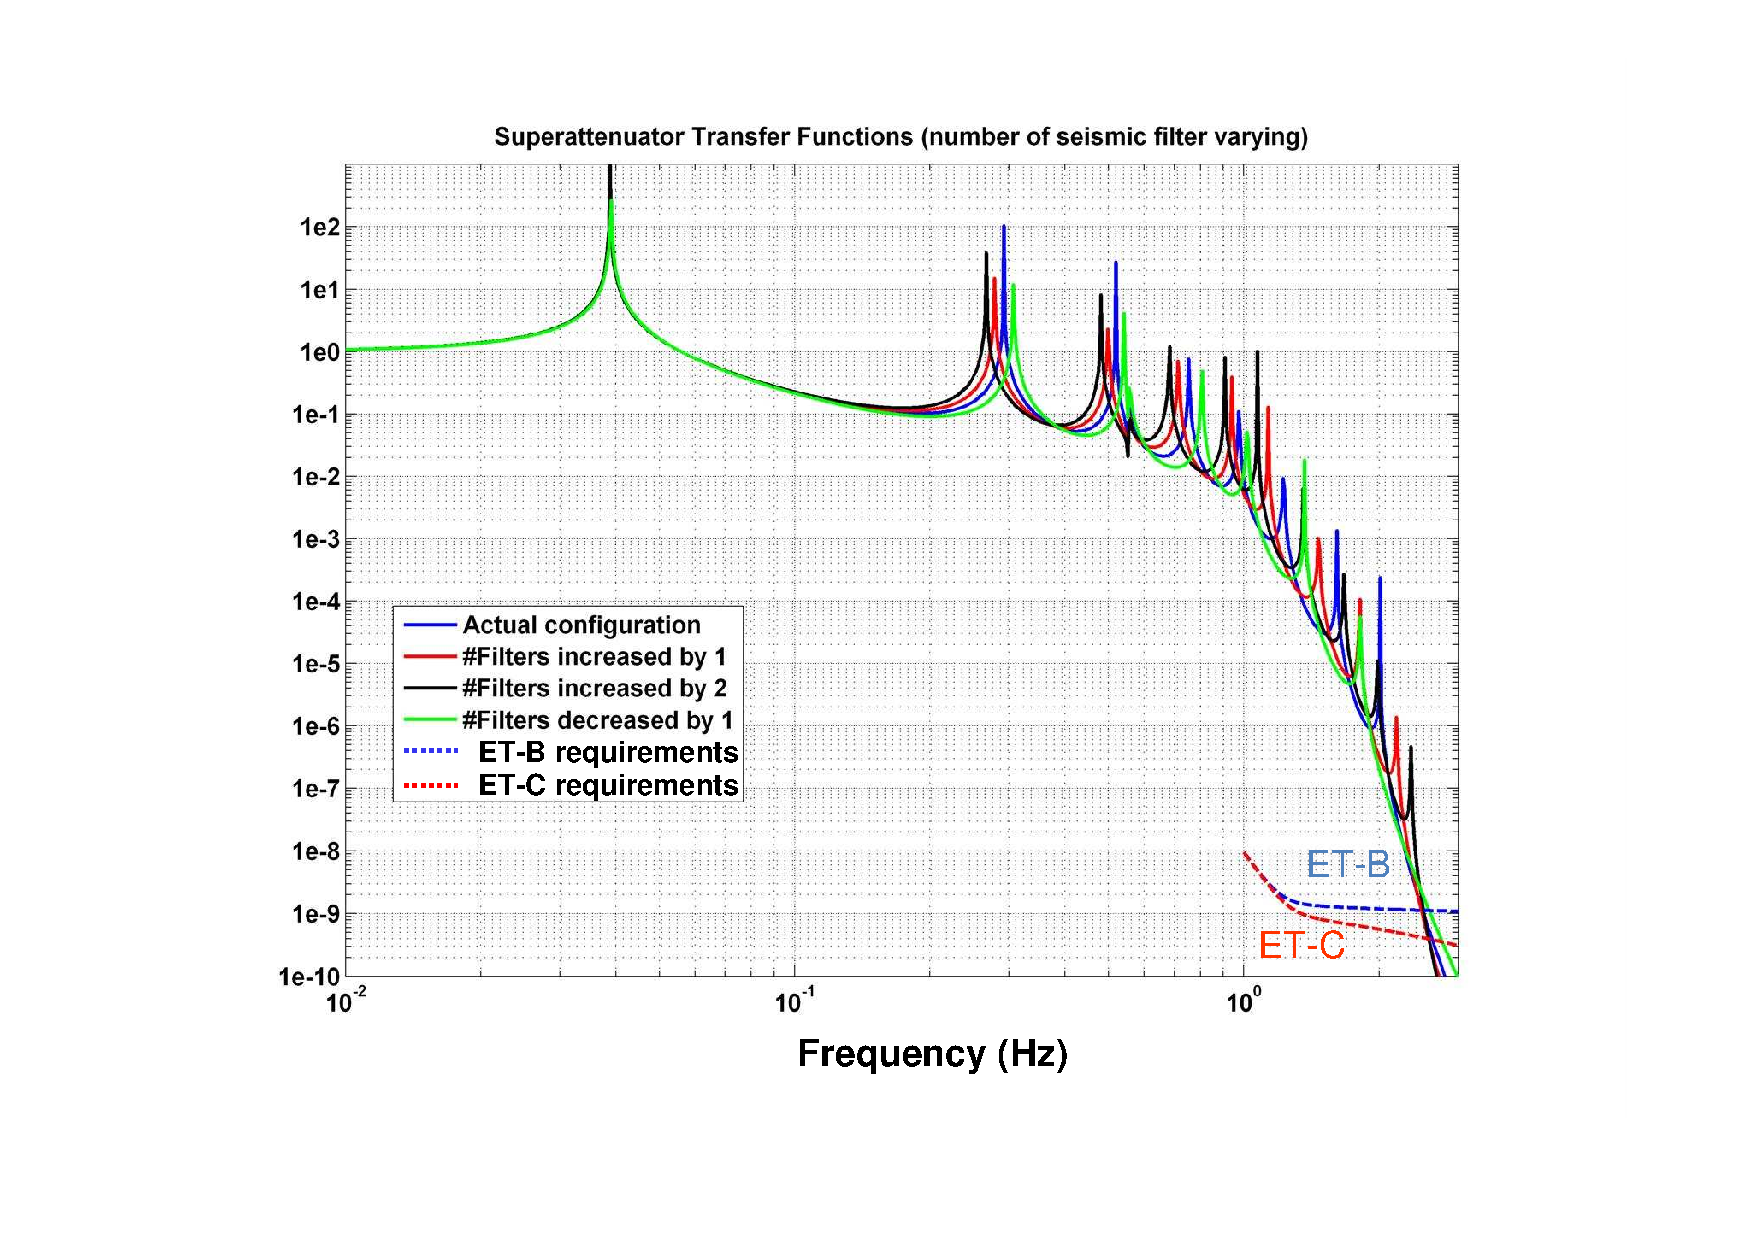
\includegraphics[width=0.9\textwidth]{Detector/SASandSUS/SuspensionSystems/Suspension_Figures/Par4-Fig1.pdf}
			\caption{Simulation results of the SA horizontal transfer function with the present chain length (9 m). Changing the number of (``equal-spaced'') filters the resulting horizontal transfer function is compared with the ET requirements (for High Frequency---\emph{ET-B}---and low frequency or ``xylophone'' configuration---\emph{ET-C}). Adding or removing filters along the chain length do not have remarkable role in the positioning of the cross-over frequency with the requirements.}
\label{Par4Fig1}
	\end{center}
\end{figure}
%
An important preliminary conclusion of the abovementioned design study is that, fixing the length and the number of mechanical filters, the optimal configuration (i.e.\ that one minimizing the cross-over frequency or maximizing the attenuation performance at 2\,Hz) is that one where the filters are separated along the chain by the same distance. This "equal-spaced" configuration represents the optimal one even because the vertical transfer function is not influenced by the filter positioning along the chain. Moreover it has been proved that increasing\,/\,decreasing the number of filters or changing their masses does not play a fundamental role in determining the cross-over frequency between the horizontal transfer function and the requirements. The results obtained are plotted in Fig.~\ref{Par4Fig1} and Fig.~\ref{Par4Fig2} while in the corresponding captions complementary information is available.  
%
\begin{figure}[t]
	\begin{center}
		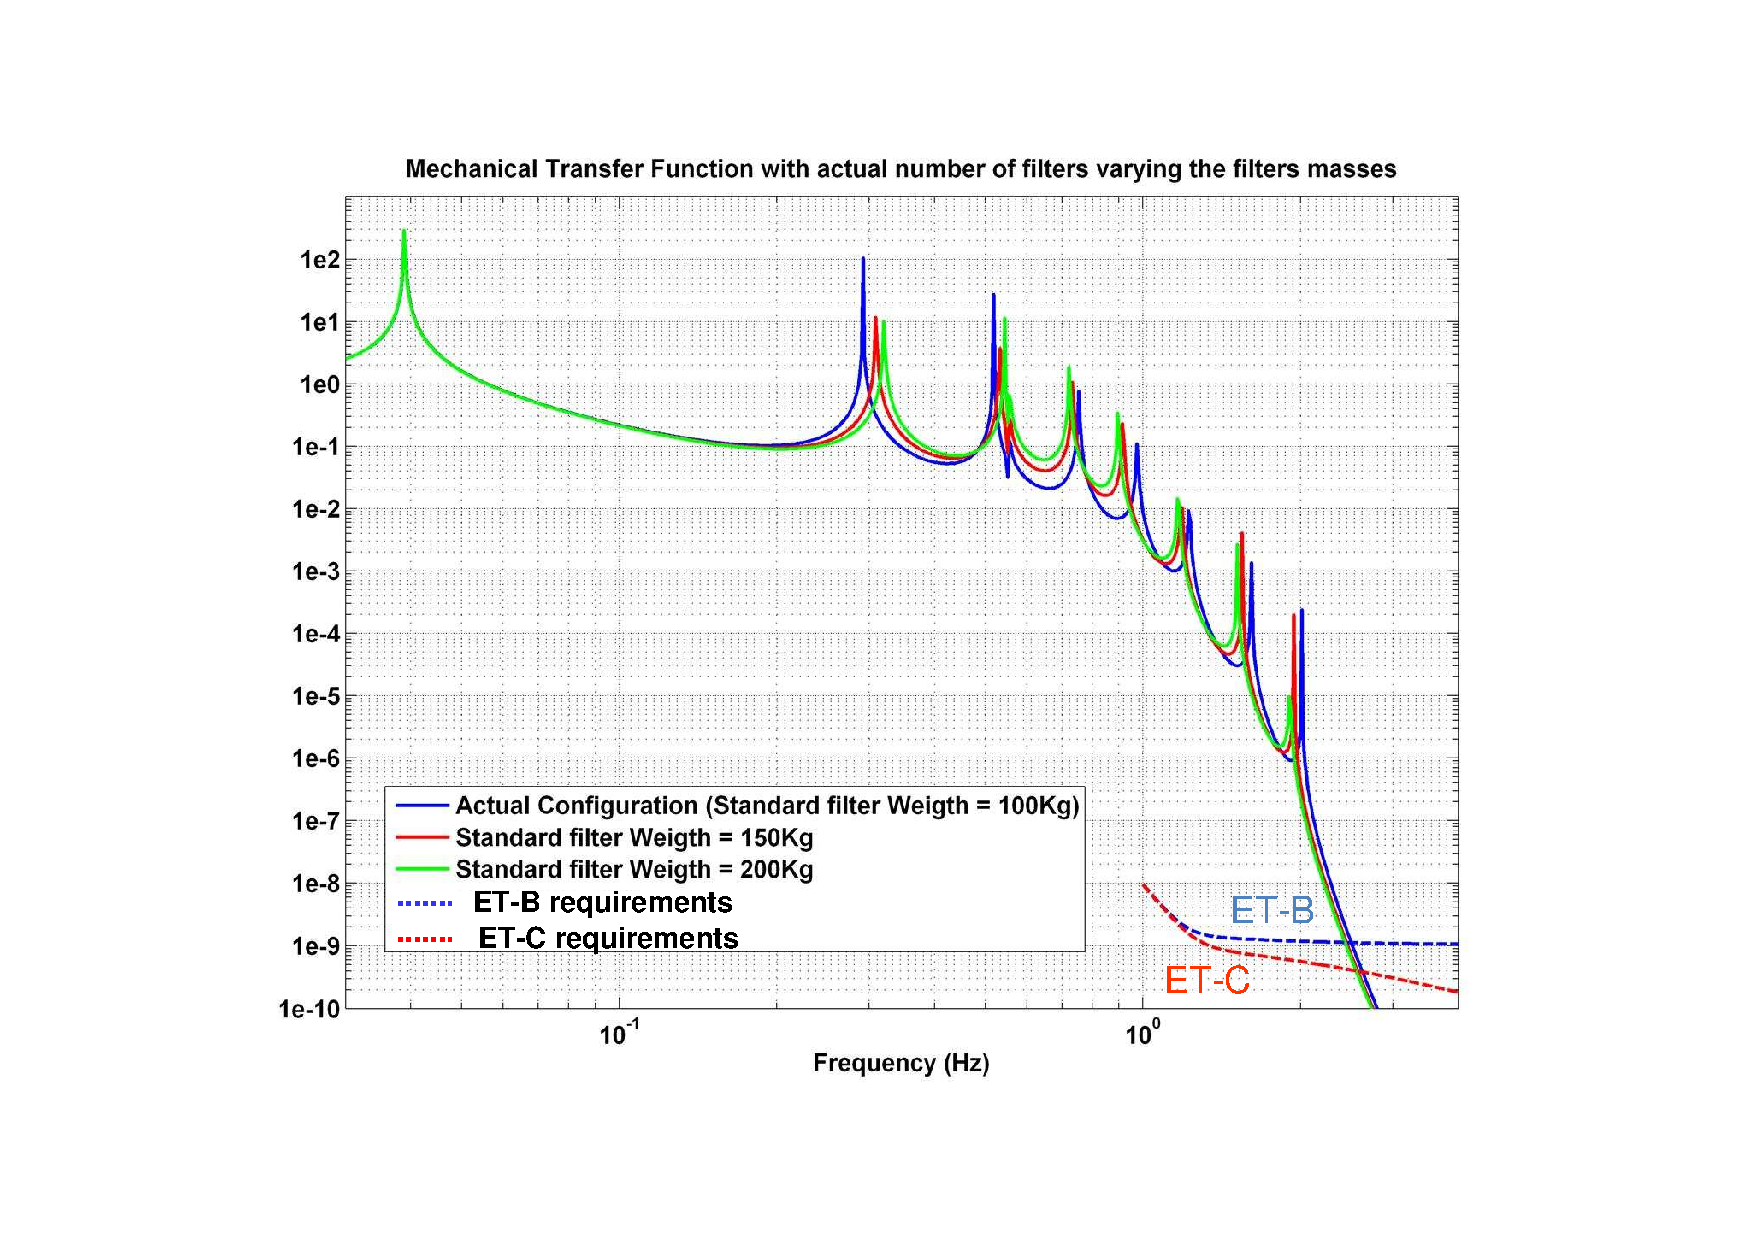
\includegraphics[width=0.9\textwidth]{Detector/SASandSUS/SuspensionSystems/Suspension_Figures/Par4-Fig2.pdf}
			\caption{The horizontal transfer function of the present \emph{SA} (6 filters weighting 100\,kg each one for a total length of about 9\,m) is compared with the same transfer function changing the mass of each filter (150\,kg and 200\,kg). Also in this case the cross-over frequency with the ET requirements is not remarkably affected by the change of the filter mass.}
\label{Par4Fig2}
	\end{center}
\end{figure}
%
\begin{figure}[t]
	\begin{center}
		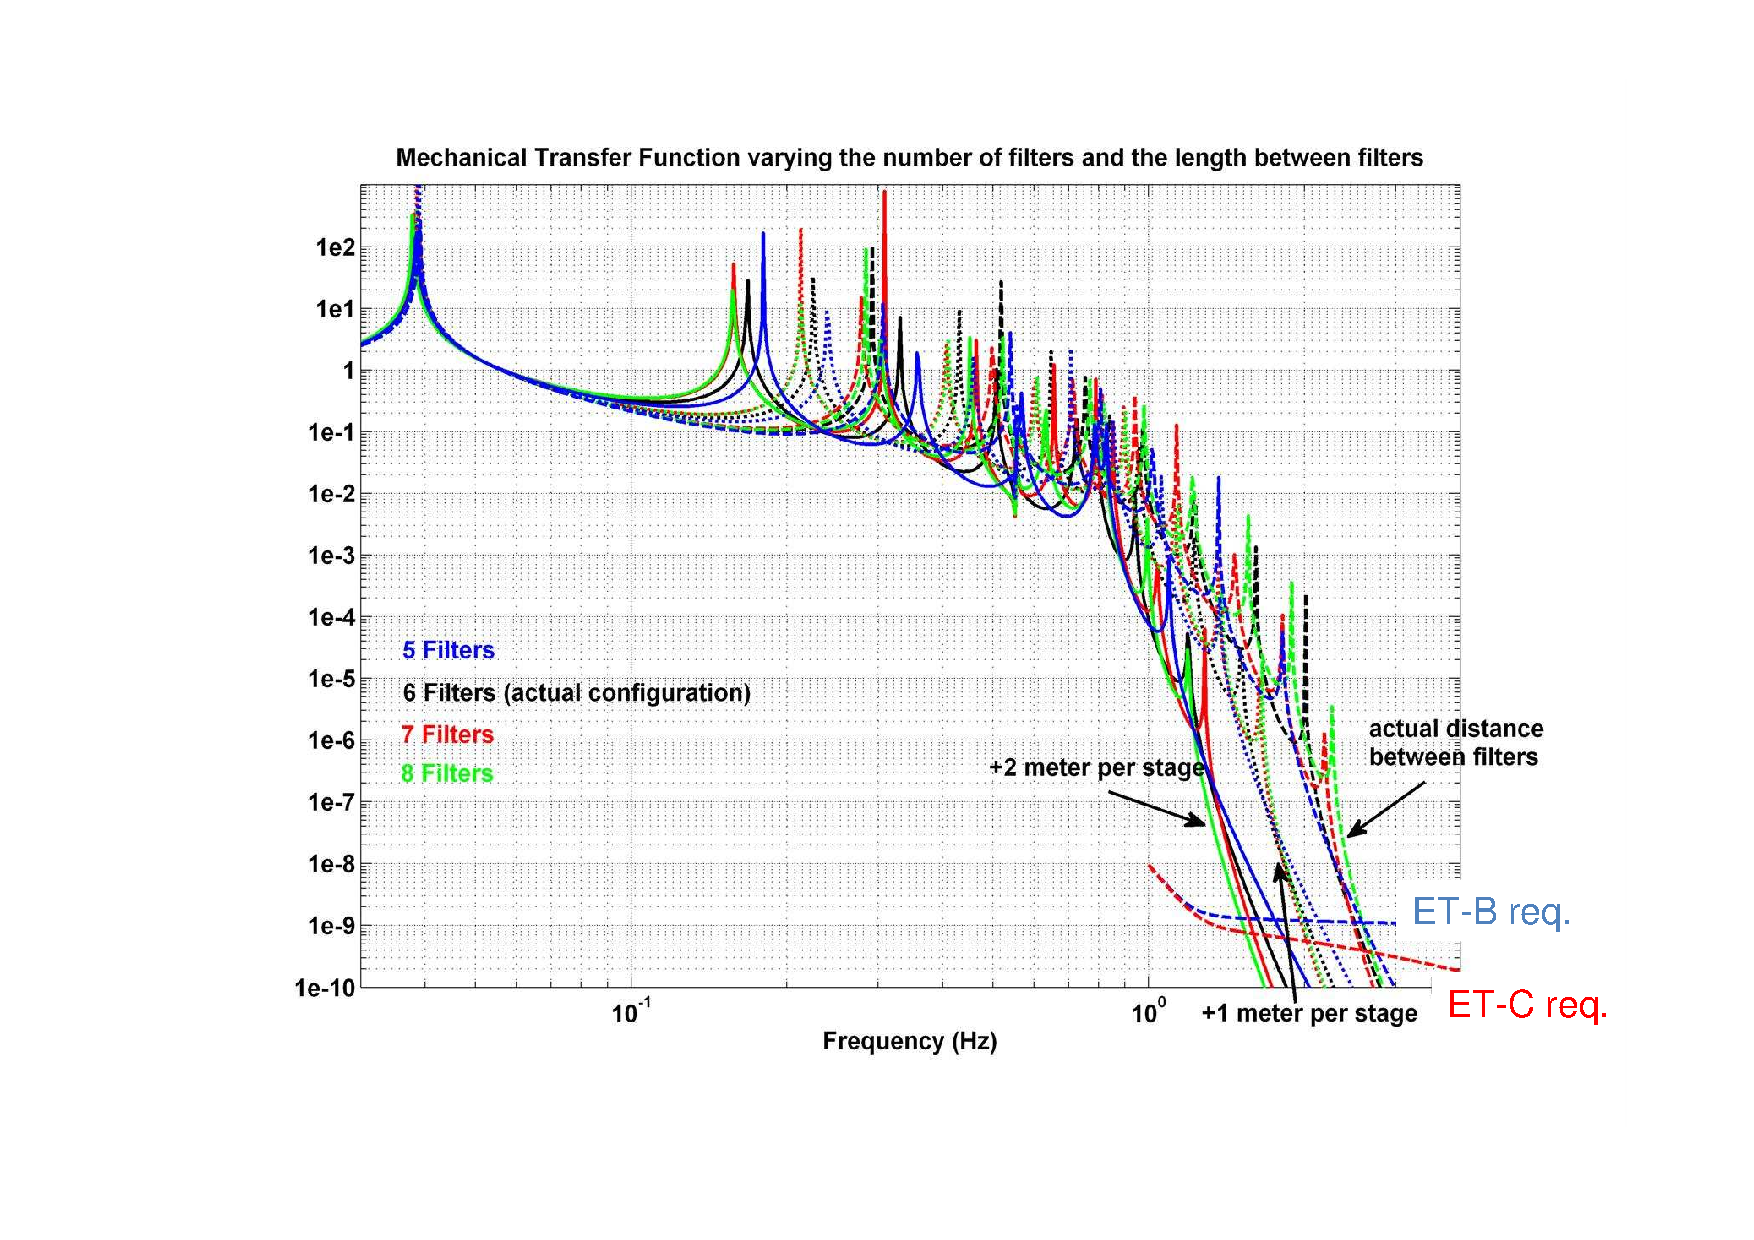
\includegraphics[width=0.9\textwidth]{Detector/SASandSUS/SuspensionSystems/Suspension_Figures/Par4-Fig3.pdf}
			\caption{Simulation results for different configurations. The horizontal transfer function of the \emph{SA} is plotted changing the number of filters and keeping fixed their relative distances ("equal-spaced" geometry) along the chain (changing, as a consequence, the full length of the SA).}
\label{Par4Fig3}
	\end{center}
\end{figure}
%
The only way to move in the low frequency region the cross-over frequency extending the Einstein Telescope bandwidth below 3 Hz, is to increase the SA chain total length. The simulation results for different configurations can be found in figure~\ref{Par4Fig3} and described in~\cite{Braccini2010March1-3}, while the best solution seems to be represented by a SA with 6 filters and a total length of 17\,m (identical the Virgo configuration, where 5 mechanical filters suspended from an horizontal pre-isolator stage plus the marionette are assembled forming a filter chain about 9\,m long). As shown in Fig.~\ref{Par4Fig4}, with this solution the cross-over frequency has been placed around 1.7--1.8\,Hz, that is considered enough for our purpose. Indeed, Newtonian noise and other technical noise are assumed to prevent an effective detection above a couple of Hz.
%
\begin{figure}[t]
	\begin{center}
		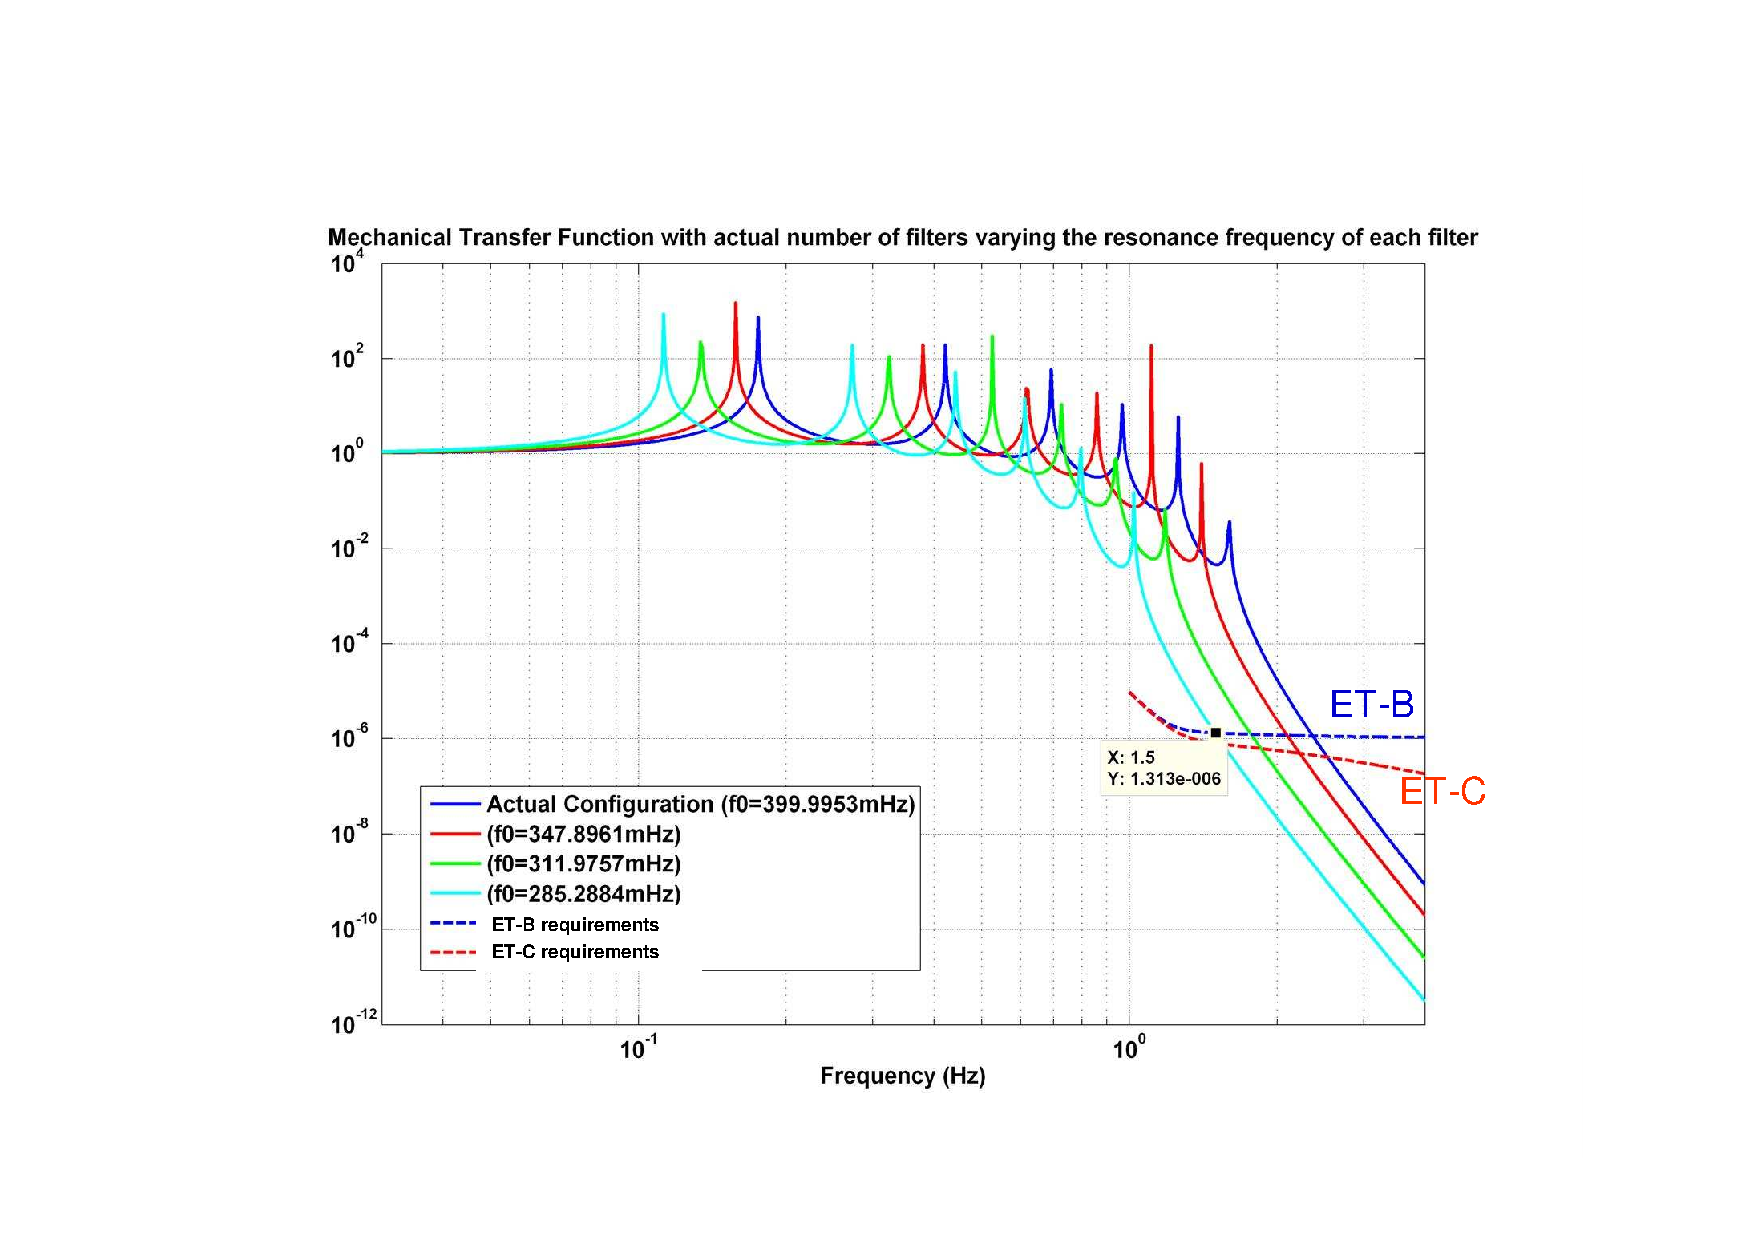
\includegraphics[width=0.9\textwidth]{Detector/SASandSUS/SuspensionSystems/Suspension_Figures/Par4-Fig5.pdf}
			\caption{Vertical Transfer Function of the SA considering the six stages (as it is now, i.e.\ with the pre-isolator or ``Filter Zero'' plus other five mechanical filters). The different curves have been obtained changing the filter vertical resonant frequency. With filters working around 300\,mHz it is possible to move the cross-over below 2\,Hz.}
\label{Par4Fig5}
	\end{center}
\end{figure}
%
With this configuration, the vertical cut-off frequency of the whole system is set below 1.8\,Hz by tuning each mechanical filter having the main vertical frequency around 300\,mHz (see Fig.~\ref{Par4Fig5}). The corresponding vertical transfer function is plotted in Fig.~\ref{Par4Fig4}. Since the residual seismic noise along the vertical direction, at the level of the mirror, is expected to limit the Einstein Telescope sensitivity again around 1.7--1.8\,Hz, a coupling factor of $10^{-3}$ has been considered. This is due to the fact that the Earth curvature makes plumb lines at a 10\,km distance not parallel each other. At least one mirror has to be inclined with respect to the local plumb line performing the alignment of the cavities. This transmits the residual vertical mirror motion along the beam with the mentioned coupling factor ($10^{-3}$).
%
\begin{figure}[t]
	\begin{center}
		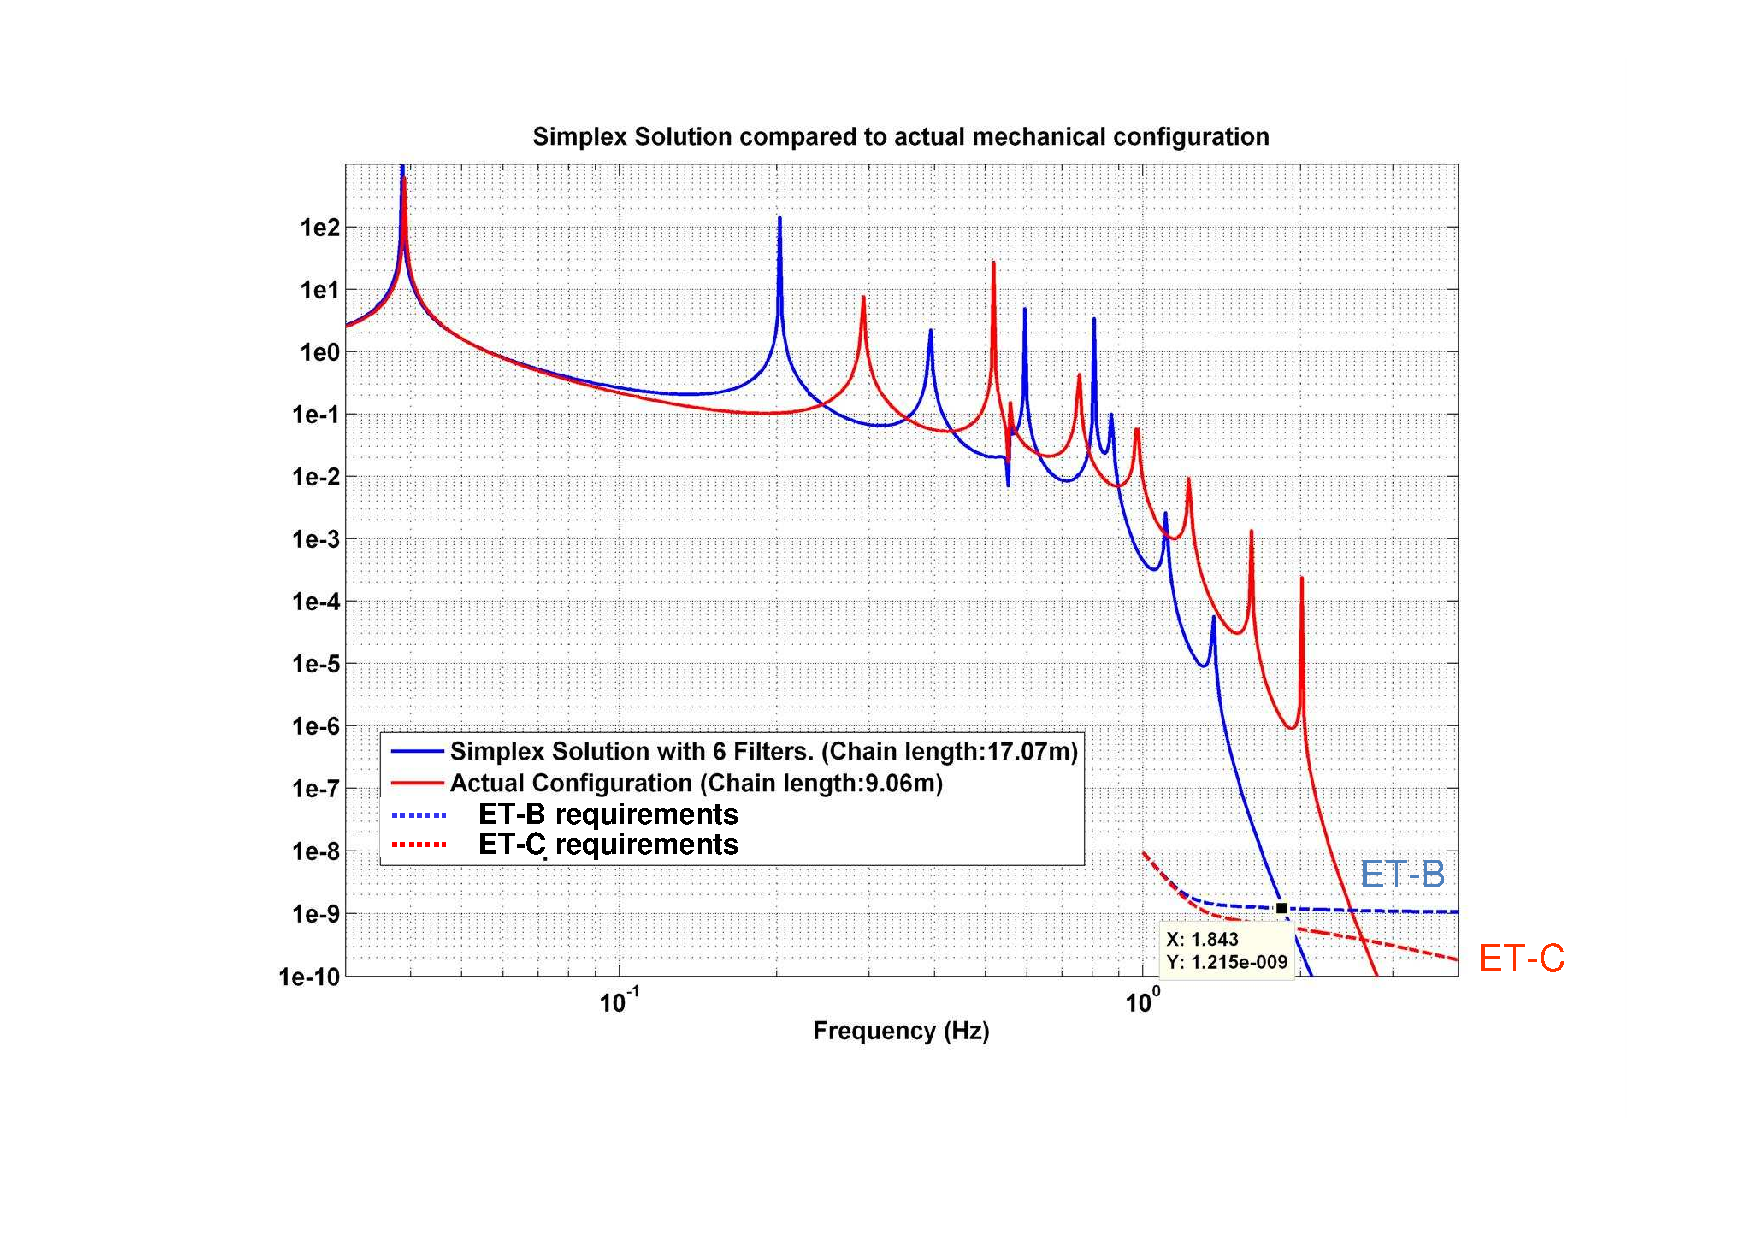
\includegraphics[width=0.9\textwidth]{Detector/SASandSUS/SuspensionSystems/Suspension_Figures/Par4-Fig4.pdf}
			\caption{The proposed reference solution for the $SA$ configuration of the Einstein Telescope. Other slightly different configurations are discussed in \cite{Braccini2010March1-3}.}
\label{Par4Fig4}
	\end{center}
\end{figure}
%
Since years in Virgo many mechanical filters with a cut-off frequency of around $300$ $mHz$ \emph{Superattenuators} are  in operation  with an excellent stability. By using the Virgo interferometer data, it has been observed that the long-term change of the chain main resonant frequencies induced by the temperature variation under vacuum are 
well inside the line-width of the chain vertical resonances. No effect on the interferometer control is due to this potential disturbance. Moreover, even if the temperature variations induce a motion of the suspension chain and then a slow vertical displacement ({\it {breath}}) of the mirror (a few $mm$ per $^{\circ}C$ is the measured 
value for the Virgo \emph{Superattenuator}), this effect is well within the specifications of any interferometer (vacuum tank provides an excellent temperature stability - fraction of $^{\circ}C$ peak to peak).
The standard SA, presently in operation on the Virgo interferometer, is already well inside the third generation specifications from this point of view too.

In addition, it is important to remind that the requirements in the tens of Hz range are less stringent in Einstein Telescope than in Advanced Virgo (see section 4.1.1.a) and thus, fixing to six (a choice lead by the reduction of the cross-over frequency) the number of filters, a better attenuation performance in the high frequency range is not necessary anymore since the safety margin is large enough in Advanced Virgo and even larger in an underground environment. In conclusion, a SA $17$ $m$ high with 6 magnetic anti-spring filters ("equal-spaced" configuration) tuned with a vertical cut-off frequency around 300 $mHz$, represents the reference solution for the Einstein Telescope. 

{\bf Possible alternatives to the baseline}

There are two main reasons which push for seeking a different approach:
\begin{itemize}
    \item the 17m Superattenuator is not sufficient to push the seismic wall down to 1 Hz, which is the ET target;
    \item it could be convenient to reduce the Superattenuator height to ease the constraints on the height of the caverns.
\end{itemize}


A possible alternative to be investigated could be coupling a Superattenuator to an inertial platform controlled in 6 d.o.f.: this configuration would make use of a combination of the technologies and expertise developed in the GW field so far. One could imagine, for instance, the inertial platform being the base of the Superattenuator. This kind of approach was envisaged already in Virgo: the Superattenators are realized on a rigid platform resting on 3 elastic feet which can be actuated by piezos. This had been designed in order to be able to perform an active control of the ground tilt. The ET design should extend this concept in order to allow also for horizontal control.




%{\bf Mechanics of the suspension upper stages}

%The suspension upper-stages are primarily required for the reduction of input vibration within the sensitive band. They are also often used for actuation and damping. 

%\textit{In Virgo, this is all filters between Filter Zero and the Marionette, in LIGO this is the 'top' and 'UIM' masses of the Quads.}



{\bf Sensor development}

The seismic isolation systems will require the development of new sensors not currently deployed in-vacuum. At the minimum, this will include some kind of inertial rotation sensor to enable tilt-control at frequencies at and below the micro-seismic peak, and displacement sensors to allow damping of suspension modes without injecting noise.
In general, the lower seismic noise intensity in the underground site will naturally require accelerometers with a lower proper noise. 

